\documentclass[11pt,a4paper]{article}

\usepackage[T1]{fontenc}
\usepackage[utf8]{inputenc}
\usepackage[protrusion=true,expansion=false]{microtype}
\usepackage[margin=2.5cm]{geometry}
\usepackage{amsmath,amssymb}
\usepackage{graphicx}
\usepackage{booktabs}
\usepackage{caption}
\usepackage{subcaption}
\usepackage[hidelinks]{hyperref}
\usepackage{enumitem}

\captionsetup{font=small,labelfont=bf}
\setlist{itemsep=2pt,topsep=4pt}

\title{\vspace{-1.5cm}\textbf{Calibration of Probabilities}\\[0.3em]
\large Assignment 2 --- Experimental Project}
\author{Behrad Sadeghi \\ \small Matricola 70193A}
\date{\small Statistical Methods for Machine Learning\\
Università degli Studi di Milano --- A.Y. 2025/26\\[0.5em]
\today}

\begin{document}
\maketitle

\begin{center}
\small
Code and results: \url{https://github.com/Behradsadeghi/ml-calibration-project}
\end{center}

\vspace{0.5em}
\hrule
\vspace{0.6em}

\noindent\small\textit{I declare that this material, which I now submit for assessment, is entirely my own
work and has not been taken from the work of others, save and to the extent that such work has been
cited and acknowledged within the text of my work. I understand that plagiarism, collusion, and copying
are grave and serious offences in the university and accept the penalties that would be imposed should I
engage in plagiarism, collusion or copying. This assignment, or any part of it, has not been previously
submitted by me or any other person for assessment on this or any other course of study.}
\normalsize

\vspace{0.6em}
\hrule
\vspace{1em}

\section{Introduction}

Supervised learning is usually presented through risk minimisation: a model is trained to minimise a
surrogate loss, and is then judged by classification accuracy. In many applications this is not enough.
A medical triage system that outputs $0.8$ should be right about $80\%$ of the time it says $0.8$;
otherwise a downstream decision rule that thresholds on cost cannot be trusted. A model with this
property is called \emph{calibrated}, and calibration is a genuinely different property from accuracy:
because Platt scaling and isotonic regression are monotonic transformations of the score, they leave the
ranking (and therefore AUC) untouched while changing the probabilities substantially.

This project reproduces, on a small scale, the study of Niculescu-Mizil and Caruana~\cite{nm2005}. Two
off-the-shelf classifiers (Logistic Regression and Random Forest) are trained on two real-world datasets;
their raw probability estimates are then post-processed with two calibration methods --- Platt scaling
and isotonic regression --- both implemented from scratch. Results are evaluated with accuracy, log-loss
and Brier score, and visualised with reliability diagrams.

The main contributions of this report, beyond the required experiments, are: (i) a multi-seed robustness
check showing that several conclusions drawn from a single split do not survive repetition; (ii) a signed
statistic that identifies the \emph{direction} of miscalibration, not only its magnitude; and (iii) an
honest account of a case where the calibration methods did not help, and of why that is the expected
outcome for these two model families.

\section{Datasets and why they were chosen}

The assignment requires two real-world classification datasets and a comparison across them. I chose two
that differ in the two properties that most directly drive calibration behaviour: how separable the
classes are, and how noisy the labels are.

\begin{table}[h]
\centering
\small
\begin{tabular}{lll}
\toprule
 & \textbf{Breast Cancer Wisconsin} & \textbf{Pima Indians Diabetes} \\
\midrule
Source & \texttt{sklearn.datasets} & OpenML \texttt{data\_id=37} (UCI mirror) \\
Samples / features & 569 / 30 & 768 / 8 \\
Positive rate & $\approx 37\%$ (malignant) & $\approx 35\%$ (tested positive) \\
Separability & high ($\approx 97\%$ test accuracy) & moderate ($\approx 76\%$ test accuracy) \\
\bottomrule
\end{tabular}
\caption{The two datasets. Both are binary and small-to-medium scale, as required.}
\end{table}

Breast Cancer is an ``easy'', well-separated problem, so I expected both models to start out close to
calibrated: it serves as a low-miscalibration reference point. Diabetes is noisier and less separable, so
I expected more miscalibration and more room for the calibration methods to help. As Section~\ref{sec:limits}
shows, that second expectation was only partly borne out --- which is itself an informative result.

The Diabetes data uses $0$ as a placeholder for missing measurements in five clinical features (glucose,
blood pressure, skin thickness, insulin, BMI), which is not physiologically valid. These zeros are treated
as missing and median-imputed using statistics computed on the training split only.

\section{Methodology}

\subsection{Splitting protocol}

Each dataset is split into three disjoint, stratified parts: $60\%$ training, $20\%$ calibration, $20\%$
test. Stratification preserves the positive rate across all three parts, which matters for the imbalanced
Diabetes data.

The separate calibration split is essential rather than cosmetic. Platt scaling and isotonic regression
are themselves fitted to data. Fitting them on the training split would correct the base model's
\emph{training-set} overconfidence rather than its generalisation behaviour; fitting them on the test
split would leak test labels into the model and inflate every reported number. Only a third, held-out
split gives an honest estimate. The same reasoning applies to feature standardisation and to median
imputation, both of which are fitted on the training split alone.

\subsection{Base models}

Logistic Regression and Random Forest ($300$ trees) are used off-the-shelf from scikit-learn, as the
assignment permits. Their hyperparameters are not the object of study: they are used purely as sources of
imperfectly calibrated probabilities. Both calibrators are fitted on top of each model's raw
\texttt{predict\_proba} output rather than a decision function, so that the two methods are applied
identically to both models even though a Random Forest has no natural margin. I tested the alternative
(applying Platt scaling to the log-odds of the probability) and it was clearly worse on Breast Cancer
(mean log-loss $0.108$ vs.\ $0.086$ for Logistic Regression) and marginally better on Diabetes, so the
simpler choice was kept.

\subsection{Platt scaling (from scratch)}

Platt scaling fits a two-parameter sigmoid on top of the raw score $f$:
\begin{equation}
P(y=1 \mid f) = \frac{1}{1 + \exp\!\big(-(Af + B)\big)} .
\end{equation}
Platt's original paper~\cite{platt1999} writes this as $1/(1+\exp(Af+B))$, in which a well-behaved fit
has $A$ negative; I use the standard logistic parameterisation above, in which $A$ is positive (typically
$A \approx +5$ in these experiments). The two are equivalent under $A \to -A$, $B \to -B$ and give
identical probabilities.
The parameters $(A,B)$ are chosen by maximum likelihood, which is convex, and are found with a
hand-written Newton's method (closed-form inverse of the $2\times2$ Hessian). Only two parameters are
fitted, which makes the method extremely data-efficient but restricts it to monotonic, sigmoid-shaped
corrections.

Crucially, the regression targets are not the raw labels $\{0,1\}$ but the Bayesian-smoothed values
\begin{equation}
t_i = \frac{N_+ + 1}{N_+ + 2} \text{ if } y_i = 1, \qquad
t_i = \frac{1}{N_- + 2} \text{ if } y_i = 0 ,
\end{equation}
where $N_+$ and $N_-$ count positives and negatives in the calibration set. Without this smoothing,
perfectly separable calibration data would drive $|A| \to \infty$ and collapse the sigmoid into a step
function. With it, the fitted probability can never reach exactly $0$ or $1$ --- a property that turns out
to matter a great deal in Section~\ref{sec:results}.

\subsection{Isotonic regression (from scratch)}

Isotonic regression solves
\begin{equation}
\min_{g \text{ non-decreasing}} \sum_i \left( y_i - g(f_i) \right)^2
\end{equation}
using the Pool-Adjacent-Violators Algorithm (PAVA), implemented as a single stack-based pass in $O(n)$
amortised time: points are sorted by score, each starts as its own block, and adjacent blocks are merged
whenever the left block's mean exceeds the right block's, re-checking backwards after each merge.

Being non-parametric, isotonic regression can represent \emph{any} monotonic correction, including shapes
a sigmoid cannot express --- but it has far more effective degrees of freedom and therefore needs more
calibration data.

For prediction I interpolate linearly between the block means rather than returning a hard step function.
This is a deliberate smoothing choice and I state it explicitly: the exactness guarantee of PAVA applies to
the fitted blocks, not to what interpolation returns, so predictions at training points are slightly worse
in residual sum of squares than the exact step solution. Scikit-learn interpolates between block
\emph{boundaries} instead and does reproduce the exact values. Both are monotonic; the difference is small.

\subsection{Metrics and visualisation}

Accuracy, log-loss, Brier score, reliability-diagram binning and Expected Calibration Error (ECE) are all
implemented from scratch with numpy. Log-loss clips probabilities to $[\varepsilon, 1-\varepsilon]$ with
$\varepsilon = 10^{-15}$, since an unclipped confidently-wrong prediction would make it infinite.

The three required metrics measure different things, which is why they can disagree. Accuracy sees only
the hard decision at threshold $0.5$ and is blind to confidence. Log-loss and Brier score are both proper
scoring rules, but log-loss is unbounded near $p \in \{0,1\}$ while Brier score is bounded in $[0,1]$ and
penalises extreme errors only quadratically. ECE, reported as a bonus, is the sample-weighted average
vertical gap between the reliability curve and the diagonal.

Reliability diagrams use ten equal-width bins and are paired with a histogram of predicted probabilities
underneath, following~\cite{nm2005}: a curve computed from a nearly empty bin is noisy, and the histogram
shows how much of the curve to trust. The binning implementation was cross-checked against
\texttt{sklearn.calibration.calibration\_curve} and agrees to $\approx 10^{-16}$.

\section{Results}
\label{sec:results}

\begin{table}[h]
\centering
\small
\begin{tabular}{llrrrr}
\toprule
\textbf{Dataset} & \textbf{Model / method} & \textbf{Accuracy} & \textbf{Log-loss} & \textbf{Brier} & \textbf{ECE} \\
\midrule
Breast Cancer & LR --- uncalibrated & 0.9649 & 0.0861 & 0.0239 & 0.0220 \\
              & LR --- Platt        & 0.9737 & 0.0885 & 0.0226 & 0.0381 \\
              & LR --- isotonic     & 0.9737 & 0.6196 & 0.0230 & 0.0245 \\
              & RF --- uncalibrated & 0.9825 & 0.1177 & 0.0296 & 0.0672 \\
              & RF --- Platt        & 0.9825 & \textbf{0.0947} & \textbf{0.0193} & 0.0468 \\
              & RF --- isotonic     & 0.9737 & 0.3606 & 0.0275 & 0.0441 \\
\midrule
Diabetes      & LR --- uncalibrated & 0.7403 & 0.5179 & 0.1743 & 0.0797 \\
              & LR --- Platt        & 0.7468 & 0.5241 & 0.1750 & 0.0528 \\
              & LR --- isotonic     & 0.6753 & 1.5688 & 0.1896 & 0.1272 \\
              & RF --- uncalibrated & 0.7208 & 0.5156 & 0.1751 & 0.0645 \\
              & RF --- Platt        & 0.7208 & 0.5227 & 0.1761 & 0.0654 \\
              & RF --- isotonic     & 0.7338 & 0.5141 & 0.1737 & 0.0464 \\
\bottomrule
\end{tabular}
\caption{Test-set metrics for the single reference split (\texttt{SEED = 42}). Lower is better for
log-loss, Brier and ECE.}
\label{tab:single}
\end{table}

\begin{figure}[h]
\centering
\begin{subfigure}{0.36\textwidth}
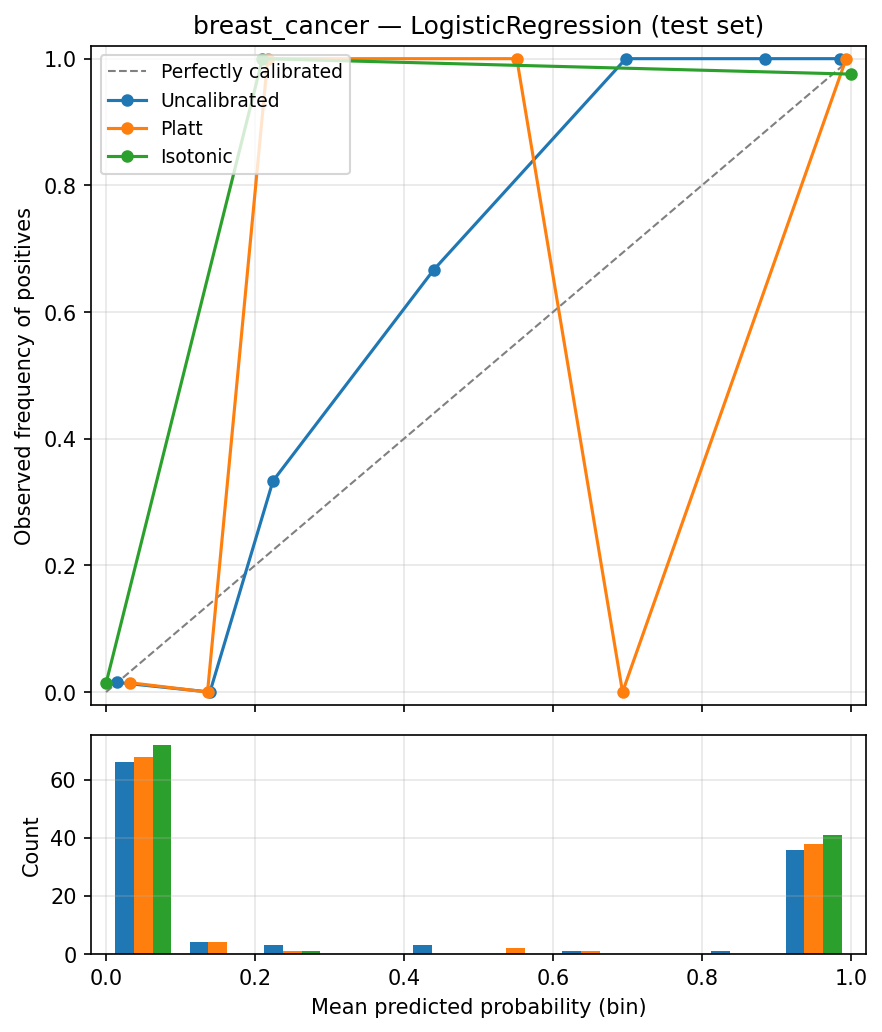
\includegraphics[width=\linewidth]{../results/plots/breast_cancer_LogisticRegression_reliability.png}
\caption{Breast Cancer, LR}
\end{subfigure}\hfill
\begin{subfigure}{0.36\textwidth}
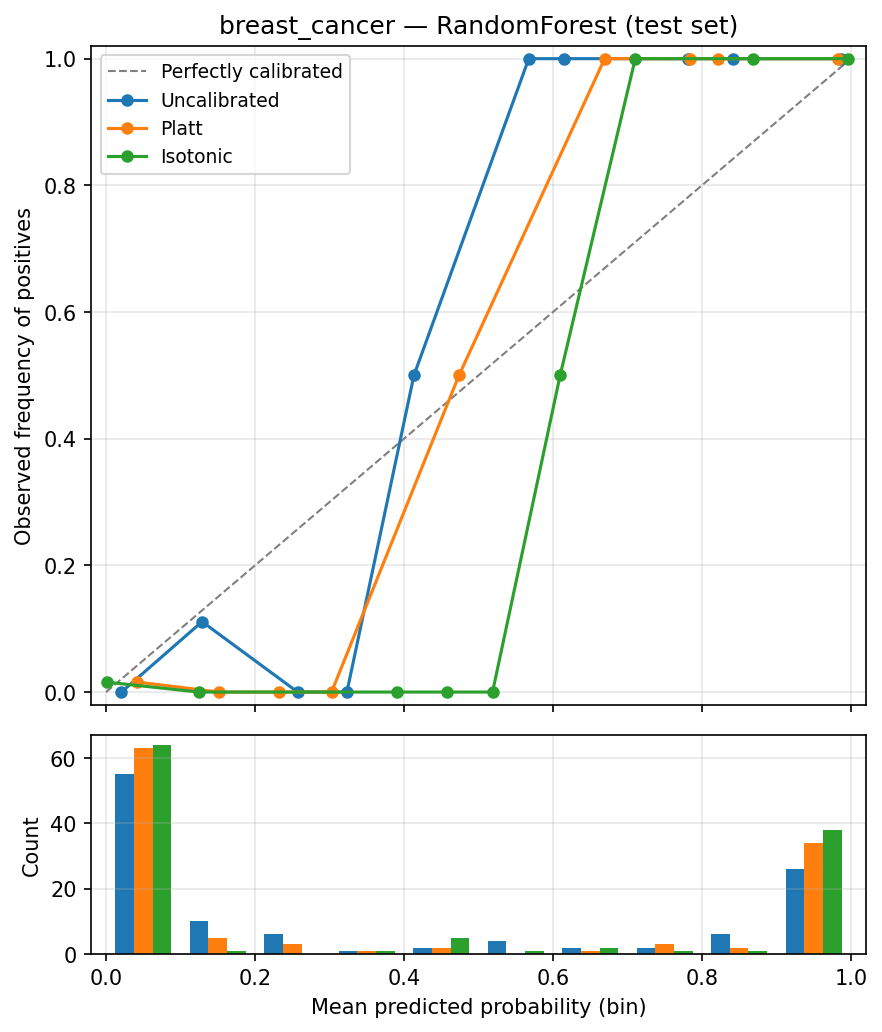
\includegraphics[width=\linewidth]{../results/plots/breast_cancer_RandomForest_reliability.png}
\caption{Breast Cancer, RF}
\end{subfigure}
\caption{Reliability diagrams before and after correction, with the histogram of predicted probabilities
below each curve. The uncalibrated Random Forest curve lies visibly off the diagonal; Platt scaling pulls
it back.}
\label{fig:rel-bc}
\end{figure}

\begin{figure}[h]
\centering
\begin{subfigure}{0.36\textwidth}
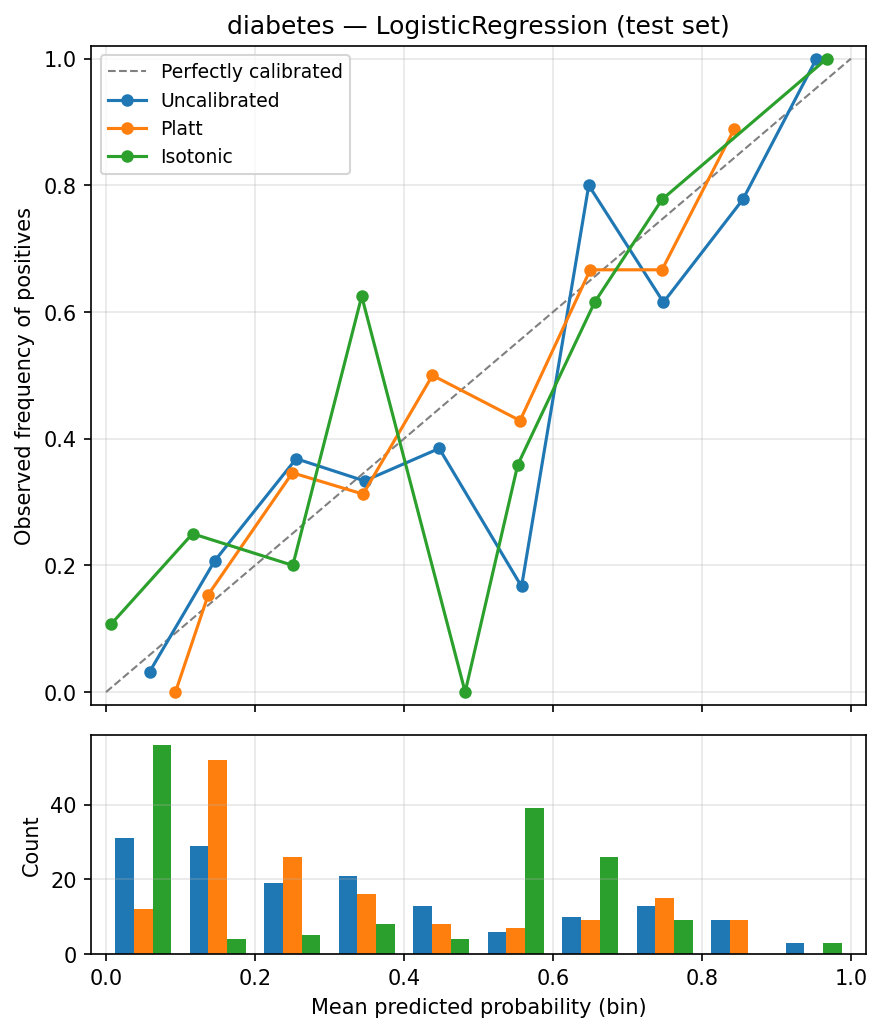
\includegraphics[width=\linewidth]{../results/plots/diabetes_LogisticRegression_reliability.png}
\caption{Diabetes, LR}
\end{subfigure}\hfill
\begin{subfigure}{0.36\textwidth}
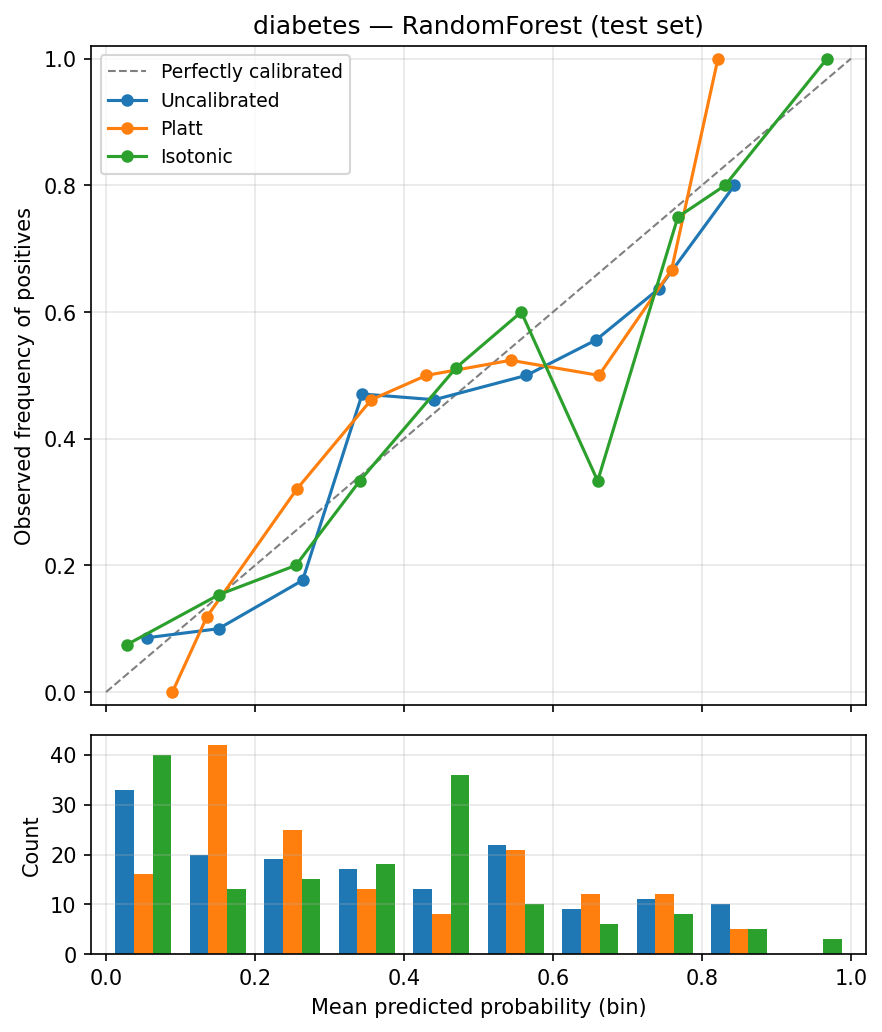
\includegraphics[width=\linewidth]{../results/plots/diabetes_RandomForest_reliability.png}
\caption{Diabetes, RF}
\end{subfigure}
\caption{Reliability diagrams on the noisier dataset. Predictions spread across the whole $[0,1]$ range
rather than bunching at the extremes, and all three curves stay closer together.}
\label{fig:rel-db}
\end{figure}

\subsection{A degenerate case for isotonic regression}

The most striking number in Table~\ref{tab:single} is the log-loss of $0.6196$ for isotonic regression on
Breast Cancer with Logistic Regression --- seven times worse than the uncalibrated baseline --- while
Brier score ($0.0239 \to 0.0230$) and accuracy ($0.965 \to 0.974$) barely move, and in fact slightly
improve.

The cause is exact and worth stating precisely. On this split the calibration set is \emph{perfectly
rank-separated} by the model's scores: every negative scores below every positive. PAVA therefore finds no
monotonicity violation to pool, each of the $114$ calibration points remains its own block, and each block
value equals that point's label --- so every fitted value is exactly $0$ or $1$. Isotonic regression has
memorised the calibration labels. This is not a bug: when the monotonicity constraint is never active, the
memorising solution \emph{is} the least-squares isotonic solution.

Two clarifications matter. First, the predictions are still piecewise linear, since I interpolate between
blocks; what collapses them onto $\{0,1\}$ is that all block values are themselves $0$ or $1$, together
with flat extrapolation outside the observed range. On this run, $113$ of the $114$ test predictions come
out at exactly $0$ or $1$. Second, only \emph{two} of those are misclassified, and those two points alone
produce the entire jump in log-loss. The magnitude is therefore sensitive to the clipping constant: the
same predictions give $0.62$ at $\varepsilon = 10^{-15}$ but $0.14$ at $\varepsilon = 10^{-3}$. The
direction of the effect is robust; the specific number should always be quoted with its $\varepsilon$.

Platt scaling is structurally immune to this failure. Its Bayesian-smoothed targets make it mathematically
impossible for the fitted sigmoid to output exactly $0$ or $1$, no matter how separable the calibration
data is. This is a concrete instance of the trade-off in~\cite{nm2005}: isotonic regression's flexibility
costs it data efficiency, and at these calibration-set sizes the cost dominates.

\section{Multi-seed robustness}

Every number in Table~\ref{tab:single} comes from one random split with $114$--$154$ calibration and test
points. That is a single sample from a noisy distribution, not an estimate. I therefore reran the entire
pipeline --- fresh split, fresh model fit, fresh calibration fit, fresh evaluation --- across ten seeds.

\begin{table}[h]
\centering
\small
\begin{tabular}{llccc}
\toprule
\textbf{Dataset} & \textbf{Model} & \textbf{Uncalibrated} & \textbf{Platt} & \textbf{Isotonic} \\
\midrule
Breast Cancer & LR & $0.085 \pm 0.029$ & $0.086 \pm 0.027$ & $0.350 \pm 0.241$ \\
Breast Cancer & RF & $0.156 \pm 0.111$ & $\mathbf{0.123 \pm 0.045}$ & $0.409 \pm 0.365$ \\
Diabetes      & LR & $0.487 \pm 0.038$ & $0.493 \pm 0.035$ & $0.803 \pm 0.344$ \\
Diabetes      & RF & $0.481 \pm 0.034$ & $0.490 \pm 0.034$ & $0.818 \pm 0.242$ \\
\bottomrule
\end{tabular}
\caption{Mean test log-loss $\pm$ standard deviation across ten random splits.}
\label{tab:multi}
\end{table}

\begin{figure}[h]
\centering
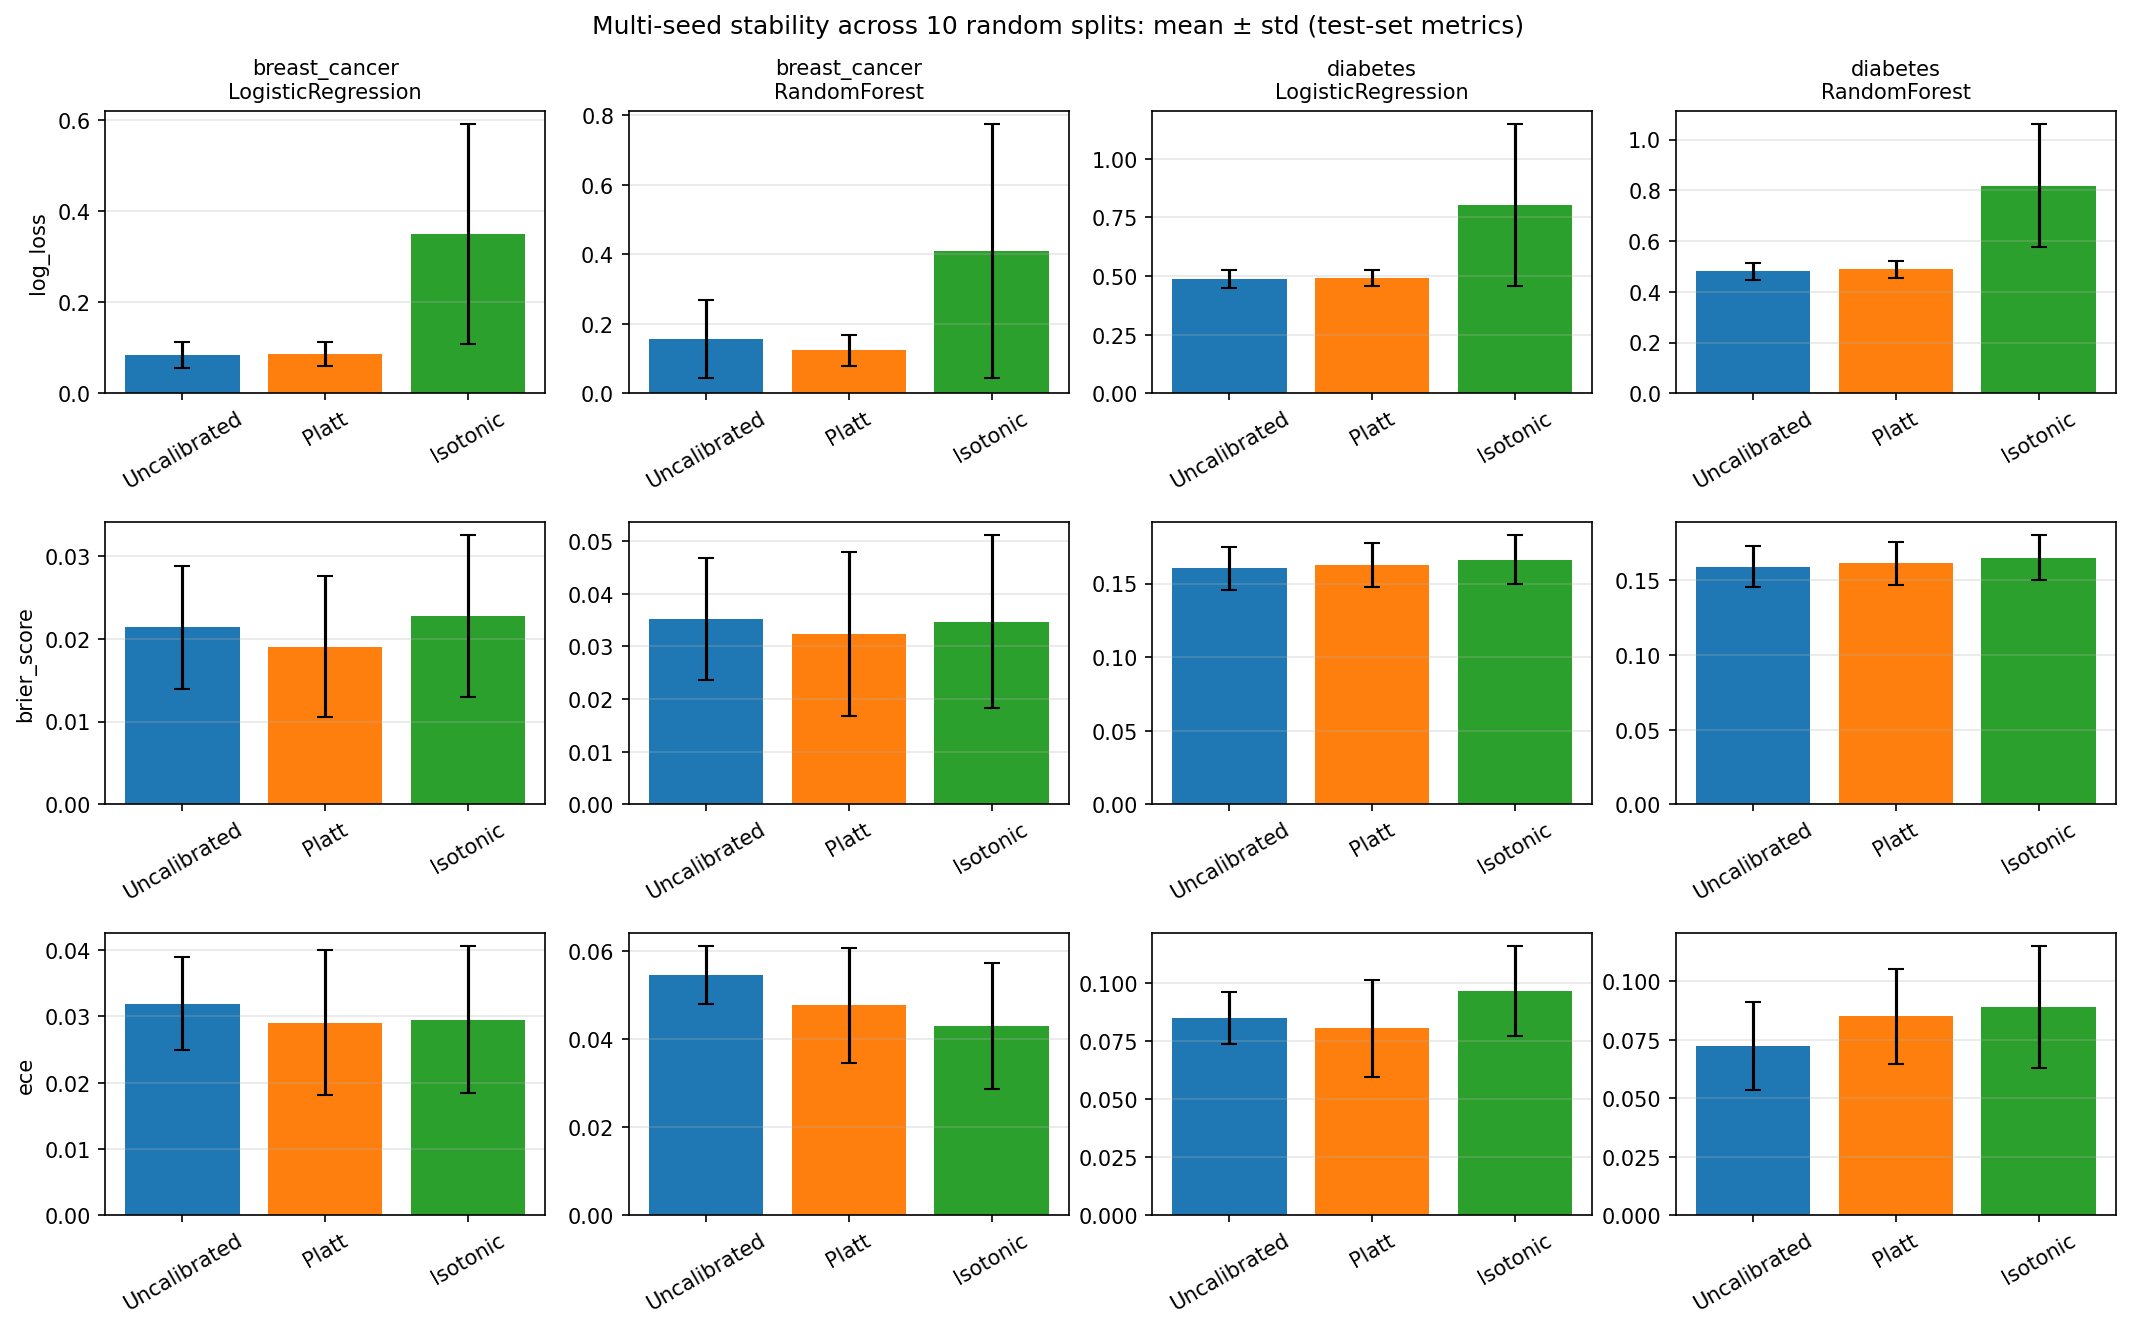
\includegraphics[width=0.95\textwidth]{../results/plots/multiseed_stability.png}
\caption{Mean $\pm$ one standard deviation across ten splits. Log-loss (top row) shows isotonic
regression's instability clearly; Brier score and ECE, being bounded, do not.}
\label{fig:multi}
\end{figure}

Two conclusions follow, and one earlier conclusion is withdrawn.

\begin{enumerate}
\item \textbf{The isotonic penalty is real and dataset-independent.} Isotonic regression's mean log-loss
exceeds Platt's in all four dataset--model combinations, not only in the degenerate Breast Cancer case.
The gap is relatively smaller on Diabetes ($\approx 1.6$--$1.7\times$ Platt's, against $3$--$4\times$ on
Breast Cancer) but it does not vanish.
\item \textbf{Its variance is large enough that single-split numbers must not be over-read.} For Random
Forest on Breast Cancer the standard deviation ($0.365$) is nearly as large as the mean ($0.409$). Notably,
Brier score and ECE show no such instability (Figure~\ref{fig:multi}): the effect is specifically an
interaction between isotonic's exact-$\{0,1\}$ outputs and log-loss's unboundedness, not a general claim
that isotonic regression is unreliable.
\item \textbf{Withdrawn:} on the single reference split it appeared that isotonic regression ``has more
room to pay off'' on the noisier dataset. Ten splits do not support this, and the claim was removed from
the analysis notebooks rather than left standing.
\end{enumerate}

\section{Discussion of miscalibration: which model, and in which direction?}

Magnitude alone does not answer the question the assignment poses. To identify \emph{direction} I use a
signed statistic, the \emph{tilt}: the sample-weighted mean gap $(\text{predicted} - \text{observed})$ over
the lower half of the probability range, minus the same quantity over the upper half. Positive tilt means
predictions are squeezed toward $0.5$ (under-confidence, curve flatter than the diagonal); negative tilt
means they are pushed away from it (over-confidence).

A plain average of $(\text{predicted} - \text{observed})$ across all bins cannot answer this, because the
positive gaps at low probabilities and the negative gaps at high probabilities cancel. Verified on
synthetic data with a known direction, that naive statistic reads $\approx 0.001$ for a strongly
under-confident model and $\approx 0.001$ for a strongly over-confident one; the tilt separates them
cleanly. Direction of miscalibration is a property of the reliability curve's \emph{slope} relative to the
diagonal, not of its average offset.

\begin{table}[h]
\centering
\small
\begin{tabular}{llcc}
\toprule
\textbf{Dataset} & \textbf{Model} & \textbf{Tilt (mean $\pm$ std)} & \textbf{Reading} \\
\midrule
Breast Cancer & LR & $+0.032 \pm 0.019$ & under-confident \\
Breast Cancer & RF & $\mathbf{+0.059 \pm 0.050}$ & under-confident, $\approx 2\times$ more than LR \\
Diabetes      & LR & $-0.060 \pm 0.115$ & no stable direction \\
Diabetes      & RF & $+0.031 \pm 0.079$ & no stable direction \\
\bottomrule
\end{tabular}
\caption{Direction of miscalibration for the uncalibrated models, across ten splits.}
\label{tab:tilt}
\end{table}

On Breast Cancer the prediction of~\cite{nm2005} holds: both models are under-confident, and the Random
Forest is roughly twice as under-confident as Logistic Regression. This is consistent with the mechanism
they describe --- averaging many de-correlated trees washes out extreme votes and pulls the ensemble's
probabilities toward the centre --- a mechanism that applies to the forest and not to the linear model.
It is also, tellingly, the one case where Platt scaling clearly helps (log-loss $0.156 \to 0.123$), which
is what one expects when there is a genuine systematic sigmoid-shaped distortion available to undo.

On Diabetes the sign flips from split to split for both models, so no honest claim about direction can be
made. Reporting the direction from the single reference split would have produced a confident-sounding
statement that ten splits do not support --- precisely the error the robustness check exists to catch.

It is also worth noting \emph{where} the miscalibration sits. Per bin, the largest gaps on Breast Cancer
occur in the middle of the probability range (roughly $0.2$--$0.7$, gaps up to $0.2$--$0.3$), while the two
outermost bins are close to calibrated (gaps of $0.003$--$0.016$). Those outermost bins hold $77$--$89\%$
of the test mass, which explains why overall ECE stays small ($0.03$--$0.05$) despite visible curvature:
the models are miscalibrated mostly in the region where they rarely predict.

\section{Limitations and negative results}
\label{sec:limits}

The most important negative result is that, across ten splits, Platt scaling improves ECE in three of four
dataset--model combinations, Brier score in two of four, and log-loss in only \emph{one} of four (Random
Forest on Breast Cancer). Isotonic regression improves none of them on log-loss. Calibration, in this
study, mostly did not help.

This is the expected outcome for these two model families, not a defect in the implementation:

\begin{itemize}
\item Logistic Regression is fitted by maximising log-likelihood --- it directly optimises a regularised
version of the very loss used to evaluate it. On a well-specified problem it is already close to
calibrated, so post-hoc correction has almost nothing to correct and mostly adds estimation noise from a
calibration set of only $110$--$150$ points.
\item Random Forest's vote-averaging \emph{is} a real, correctable distortion, and Platt scaling does
correct it --- visibly so on Breast Cancer. That combination is not the one with the largest raw
miscalibration (Diabetes has higher ECE for both models), but it is the one whose miscalibration is most
\emph{systematic}: it has the largest tilt with a stable sign across splits (Table~\ref{tab:tilt}). This
distinction matters. Platt scaling has two parameters and can only undo a distortion with a consistent
sigmoid shape; it cannot repair miscalibration that has no stable direction. On Diabetes the tilt's sign
flips from split to split, so there is more error to fix but no systematic shape to fix it with --- which
is precisely why the larger ECE there does not translate into a larger gain from calibration.
\end{itemize}

The deeper limitation is the choice of model families. The dramatic gains in~\cite{nm2005} come from
boosted trees, SVMs and Naive Bayes --- families whose scores are systematically distorted (boosting pushes
scores away from $0$ and $1$ in a characteristic sigmoidal way; SVM margins are not probabilities at all).
The assignment specifies Logistic Regression and Random Forest, which sit at the well-calibrated end of
that paper's own comparison. This study is therefore structurally unlikely to reproduce the paper's
largest effects; its results are consistent with the paper rather than contradicting it. Extending the
study with a deliberately miscalibrated base model would be the natural next step.

Two further limitations: ten seeds is enough to detect large effects and expose instability, but not to
resolve the small differences between Platt scaling and the uncalibrated baseline; and Random Forest
results shift slightly across scikit-learn versions even with a fixed \texttt{random\_state}, so exact
reproduction requires the pinned versions in \texttt{requirements.txt}.

\section{Conclusion}

Both calibration methods were implemented from scratch and behave correctly: Platt scaling agrees with an
unregularised logistic regression fitted on the same scores to within $0.005$, and the PAVA output is
monotonic by construction. The clearest experimental finding is the trade-off between the two methods.
Platt scaling's two parameters and smoothed targets make it robust at small calibration-set sizes;
isotonic regression's flexibility, valuable in principle, degenerates into label memorisation when the
calibration set is small and well separated, producing predictions of exactly $0$ or $1$ that log-loss
punishes severely while accuracy and Brier score barely register. At the sample sizes available here,
Platt scaling is the safer default on both datasets.

Equally important is what the multi-seed check revealed: a confident-sounding claim drawn from one split
did not survive repetition, and the direction of miscalibration on the noisier dataset turned out not to be
identifiable at all. For a study whose entire subject is the trustworthiness of reported probabilities,
reporting uncertainty about its own numbers seemed the minimum standard to hold.

\begin{thebibliography}{9}
\bibitem{nm2005}
A.~Niculescu-Mizil and R.~Caruana.
\newblock Predicting Good Probabilities with Supervised Learning.
\newblock \emph{Proceedings of the 22nd International Conference on Machine Learning (ICML)}, 2005.

\bibitem{platt1999}
J.~Platt.
\newblock Probabilistic Outputs for Support Vector Machines and Comparisons to Regularized Likelihood
Methods.
\newblock \emph{Advances in Large Margin Classifiers}, 1999.

\bibitem{linlin2007}
H.-T.~Lin, C.-J.~Lin and R.~C.~Weng.
\newblock A Note on Platt's Probabilistic Outputs for Support Vector Machines.
\newblock \emph{Machine Learning}, 68(3):267--276, 2007.
\end{thebibliography}

\end{document}
